\section{Pre-Training Architecture}

\subsection{Overall Architecture}

M2 is a large-scale sparse language model based on a Mixture-of-Experts (MoE) architecture, designed to scale model capacity while maintaining a low per-token compute budget. It contains 229.9B total parameters, with 9.8B activated per token. The model is implemented as a 62-layer decoder-only Transformer with a hidden dimension of 3{,}072 and a vocabulary size of 200{,}064, and is pre-trained on 29.2T tokens with a maximum context length of 192K.

Each Transformer block in M2 consists of a multi-head self-attention module followed by a Mixture-of-Experts (MoE) feed-forward layer. For attention, M2 adopts full multi-head attention across all layers, using 48 query heads and 8 key-value heads (GQA)~\citep{ainslie2023gqa}. Rotary Position Embeddings (RoPE)~\citep{su2024roformer} are applied throughout the model. This design departs from the hybrid attention mechanisms explored in MiniMax-Text-01~\citep{minimax2025minimax01} and reflects our preference for full attention in large-scale settings (Section~\ref{sec:attention-design}). The MoE feed-forward layer contains 256 fine-grained experts~\citep{dai2024deepseekmoe}, with 8 experts activated per token. Routing is implemented using sigmoid gating with learnable expert-specific bias terms, which improves load balancing while greatly reducing reliance on auxiliary losses~\citep{wang2024auxfree} (Section~\ref{sec:moe}). In addition to the standard next-token prediction objective, we incorporate a Multi-Token Prediction (MTP) module~\citep{gloeckle2024better} during pre-training. This module is expanded during continued pre-training via weight copying to support multi-step speculative decoding~\citep{leviathan2023fast} (Section~\ref{sec:mtp}).

\subsection{Model Design Choice}
\label{sec:design-choice}

M2's design space is dominated by two architectural decisions: how the feed-forward layer is sparsified, and how attention is structured across layers. Each decision was made by deliberately benchmarking against alternatives, with the rationale and supporting evidence detailed below.

\subsubsection{Mixture-of-Experts}
\label{sec:moe}

M2 employs a Mixture-of-Experts (MoE) architecture for its feed-forward layers, with three modifications targeting expressiveness, routing dynamics, and load balancing.

\noindent \textbf{Fine-Grained Experts.} We adopt a fine-grained expert design that uses a larger number of smaller experts, increasing the total expert count while reducing per-expert FFN size. This increases the combinatorial diversity of routing and reduces variance in expert utilization across devices (Table~\ref{tab:fine-grained-experts}).

\begin{table}[h]
\centering
\caption{Ablation studies for the MoE Fine-Grained Experts design and the Multi-Token Prediction (MTP) module, evaluated on \emph{MATH}~\citep{hendrycks2021math}, \emph{MMLU}~\citep{hendrycks2021mmlu}, \emph{ARC-Challenge}~\citep{clark2018arc}, \emph{KorBench}~\citep{ma2025korbenchbenchmarkinglanguagemodels}, and \emph{HumanEval}~\citep{chen2021humaneval}. Bold marks the highest score in each row.}
\label{tab:fine-grained-experts}
\label{tab:mtp-ablation}
\begin{tabular}{lcccc}
\toprule
& \textbf{Shots} & \textbf{Baseline} & \textbf{w/ MTP} & \textbf{w/ Fine-Grained} \\
\midrule
\multicolumn{5}{l}{\textit{Model Configuration}} \\
Activated Params & -- & 2B & 2B & 2B \\
Total Params & -- & 17.8B & 17.8B & 17.8B \\
Training Tokens & -- & 500B & 500B & 500B \\
\texttt{num\_experts} & -- & 32 & 32 & 128 \\
\texttt{topk} & -- & 2 & 2 & 8 \\
\midrule
\multicolumn{5}{l}{\textit{Benchmark Results}} \\
MATH & 4-shot & 19.6 & 21.3 & \textbf{24.1} \\
MMLU & 5-shot & 39.8 & 39.7 & \textbf{40.2} \\
ARC-Challenge & 25-shot & 27.4 & 27.5 & \textbf{27.8} \\
KorBench & 3-shot & 14.1 & \textbf{15.0} & 14.8 \\
HumanEval & 0-shot & 29.7 & 30.1 & \textbf{32.5} \\
\bottomrule
\end{tabular}
\end{table}

\noindent \textbf{Sigmoid Gating.} Instead of softmax-based top-$k$ gating~\citep{shazeer2017moe}, we use sigmoid gating for expert routing. Each expert receives an independent activation score, removing the zero-sum constraint imposed by softmax. This allows multiple experts to be activated simultaneously with high confidence and leads to smoother routing dynamics during training.

\noindent \textbf{Expert Bias.} We introduce learnable bias terms in the gating function as per-expert routing-score shifts. These biases are optimized jointly with model parameters and implicitly regulate expert utilization, allowing the auxiliary load-balancing loss to be greatly reduced.

\subsubsection{Attention}
\label{sec:attention-design}

M2 adopts full multi-head attention across all layers, departing from the hybrid design used in MiniMax-Text-01~\citep{minimax2025minimax01}, which interleaves Lightning Attention~\citep{qin2024lightning} with full attention. Despite the theoretical appeal of efficient attention mechanisms, we found no variant that reliably matches full attention quality in production settings spanning reasoning, coding, and agent tasks.

\noindent \textbf{Evaluation Difficulty.} The core challenge is reliably measuring quality loss. During MiniMax-Text-01 development, our hybrid attention models appeared to match full attention on standard benchmarks (\emph{MMLU}~\citep{hendrycks2021mmlu}, \emph{BBH}~\citep{suzgun2023challenging}, \emph{MATH}~\citep{hendrycks2021math}, \emph{LongBench}~\citep{bai2024longbench}), but at a larger scale, clear deficits emerged in complex multi-hop reasoning. We developed proxy metrics to address these gaps, but the correlation between proxy metrics and real downstream performance is fragile---it may not hold at larger scales or on unseen task distributions. Moreover, the compute required for statistically significant evaluation grows substantially with task complexity, and different architectures interact unpredictably with data distributions and training recipes, making reliable comparisons exceptionally difficult.

\noindent \textbf{Infrastructure Gap.} Linear and sparse attention infrastructure remains less mature than full attention. Many linear architectures are memory-bound even during training. For inference, key challenges remain: sensitivity to low-precision storage, lack of native prefix caching support, and unclear integration with speculative decoding.

\noindent \textbf{Hybrid SWA Experiments.} We extensively explored hybrid Sliding Window Attention~\citep{beltagy2020longformer} variants for M2's attention layers, continuing pre-training for hundreds of billions to trillions of tokens across multiple configurations---varying SWA/full attention ratios, adjusting RoPE settings, exploring intra-layer and inter-layer hybrids, analyzing attention patterns (induction heads~\citep{olsson2022induction}, retrieval heads~\citep{wu2024retrieval}), and adding sink tokens~\citep{xiao2024streamingllm}. During pre-training, all variants showed degraded performance on retrieval, multi-hop reasoning, and in-context learning tasks (Table~\ref{tab:swa-pretrain}). After SFT, the gap became more pronounced specifically at long context: on benchmarks exceeding 32K context (agent tasks and complex long-context evaluations), SWA variants performed significantly worse than full attention. On benchmarks within 32K, differences were mixed and small in absolute terms---SWA matched or even exceeded full attention on some instruction-following and shorter-horizon agent tasks (e.g., \emph{IFBench}, \emph{XBench-ds}), while full attention retained advantages on knowledge-intensive evaluations (e.g., \emph{GPQA-Diamond}, \emph{MMLU-Pro}); see Table~\ref{tab:swa-sft-general}. These findings suggest that hybrid SWA's attention coverage limitations critically impact long-context capabilities while having minimal effect on shorter-context scenarios.

\noindent \textbf{Outlook.} As context lengths grow and GPU compute scaling slows, sub-quadratic attention will become increasingly relevant. We are investing in better long-context data, evaluation methodologies, and infrastructure to enable this transition.

\begin{table}[h]
\centering
\caption{Pretraining evaluation at the M2 architecture scale: full attention baseline vs.\ hybrid SWA, covering general knowledge (\emph{MMLU}~\citep{hendrycks2021mmlu}, \emph{MATH}~\citep{hendrycks2021math}), long-context retrieval (\emph{HELMET}~\citep{yen2024helmet}, \emph{RULER}~\citep{hsieh2024ruler}), and in-context translation (\emph{MTOB}~\citep{tanzer2024mtob}). Bold marks the highest score in each row.}
\label{tab:swa-pretrain}
\begin{tabular}{lcc}
\toprule
& \textbf{Baseline} & \textbf{w/ SWA} \\
\midrule
HELMET ICL & \textbf{75.8} & 72.7 \\
MMLU & 85.5 & 85.6 \\
MATH & 60.3 & 60.3 \\
RULER 128K CWE & \textbf{90.0} & 72.0 \\
RULER 128K MQ & \textbf{99.0} & 93.0 \\
RULER 32K CWE & 99.0 & 99.0 \\
RULER 32K MQ & 99.0 & 99.0 \\
MTOB K-e Bleurt & \textbf{60.0} & 45.0 \\
MTOB e-k ChrF & \textbf{44.8} & 27.2 \\
\bottomrule
\end{tabular}
\end{table}

\begin{table}[h]
\centering
\caption{SFT benchmark at the M2 architecture scale: full attention baseline vs.\ hybrid SWA, covering general reasoning/knowledge and agentic tasks. General benchmarks: \emph{AIME 2025}~\citep{aime2025}, \emph{ARC-AGI-1}~\citep{chollet2019arcagi}, \emph{GPQA-Diamond}~\citep{rein2024gpqa}, \emph{MMLU-Pro}~\citep{wang2024mmlu}, \emph{IFBench}~\citep{pyatkin2025ifbench}. Agent benchmarks: \emph{SWE-verified}~\citep{jimenez2024swebench}, \emph{Terminal-Bench}~\citep{merrill2026terminalbench}, \emph{BrowseComp-zh}~\citep{zhou2025browsecompzhbenchmarkingwebbrowsing}, \emph{GAIA-103}~\citep{mialon2024gaia}, \emph{XBench-ds}~\citep{chen2025xbench}, \emph{$\tau^2$-Bench}~\citep{barres2025tau2benchevaluatingconversationalagents}. Bold marks the highest score in each row.}
\label{tab:swa-sft-general}
\begin{tabular}{lcc}
\toprule
& \textbf{Baseline} & \textbf{w/ SWA} \\
\midrule
\multicolumn{3}{l}{\textit{General Benchmarks}} \\
AIME 2025 & 86.7 & 86.7 \\
ARC-AGI-1 & 38.9 & \textbf{39.6} \\
GPQA-Diamond & \textbf{75.3} & 72.7 \\
MMLU-Pro & \textbf{80.5} & 80.1 \\
IFBench & 23.1 & \textbf{27.2} \\
\midrule
\multicolumn{3}{l}{\textit{Agent Benchmarks}} \\
SWE-verified & \textbf{54.7} & 50.2 \\
Terminal-Bench & \textbf{26.7} & 23.8 \\
BrowseComp-zh & \textbf{32.8} & 28.7 \\
GAIA-103 & \textbf{53.4} & 51.5 \\
XBench-ds & 58.0 & \textbf{63.0} \\
$\tau^2$-Bench retail & 62.3 & \textbf{67.5} \\
$\tau^2$-Bench telecom & \textbf{32.5} & 21.0 \\
\bottomrule
\end{tabular}
\end{table}

\subsection{Multi-Token Prediction}
\label{sec:mtp}

M2 incorporates Multi-Token Prediction (MTP)~\citep{gloeckle2024better}, which trains the model to predict the next $K$ tokens jointly. This design provides richer training signals and enables speculative decoding~\citep{leviathan2023fast} at inference time.

\begin{figure}[h]
\centering
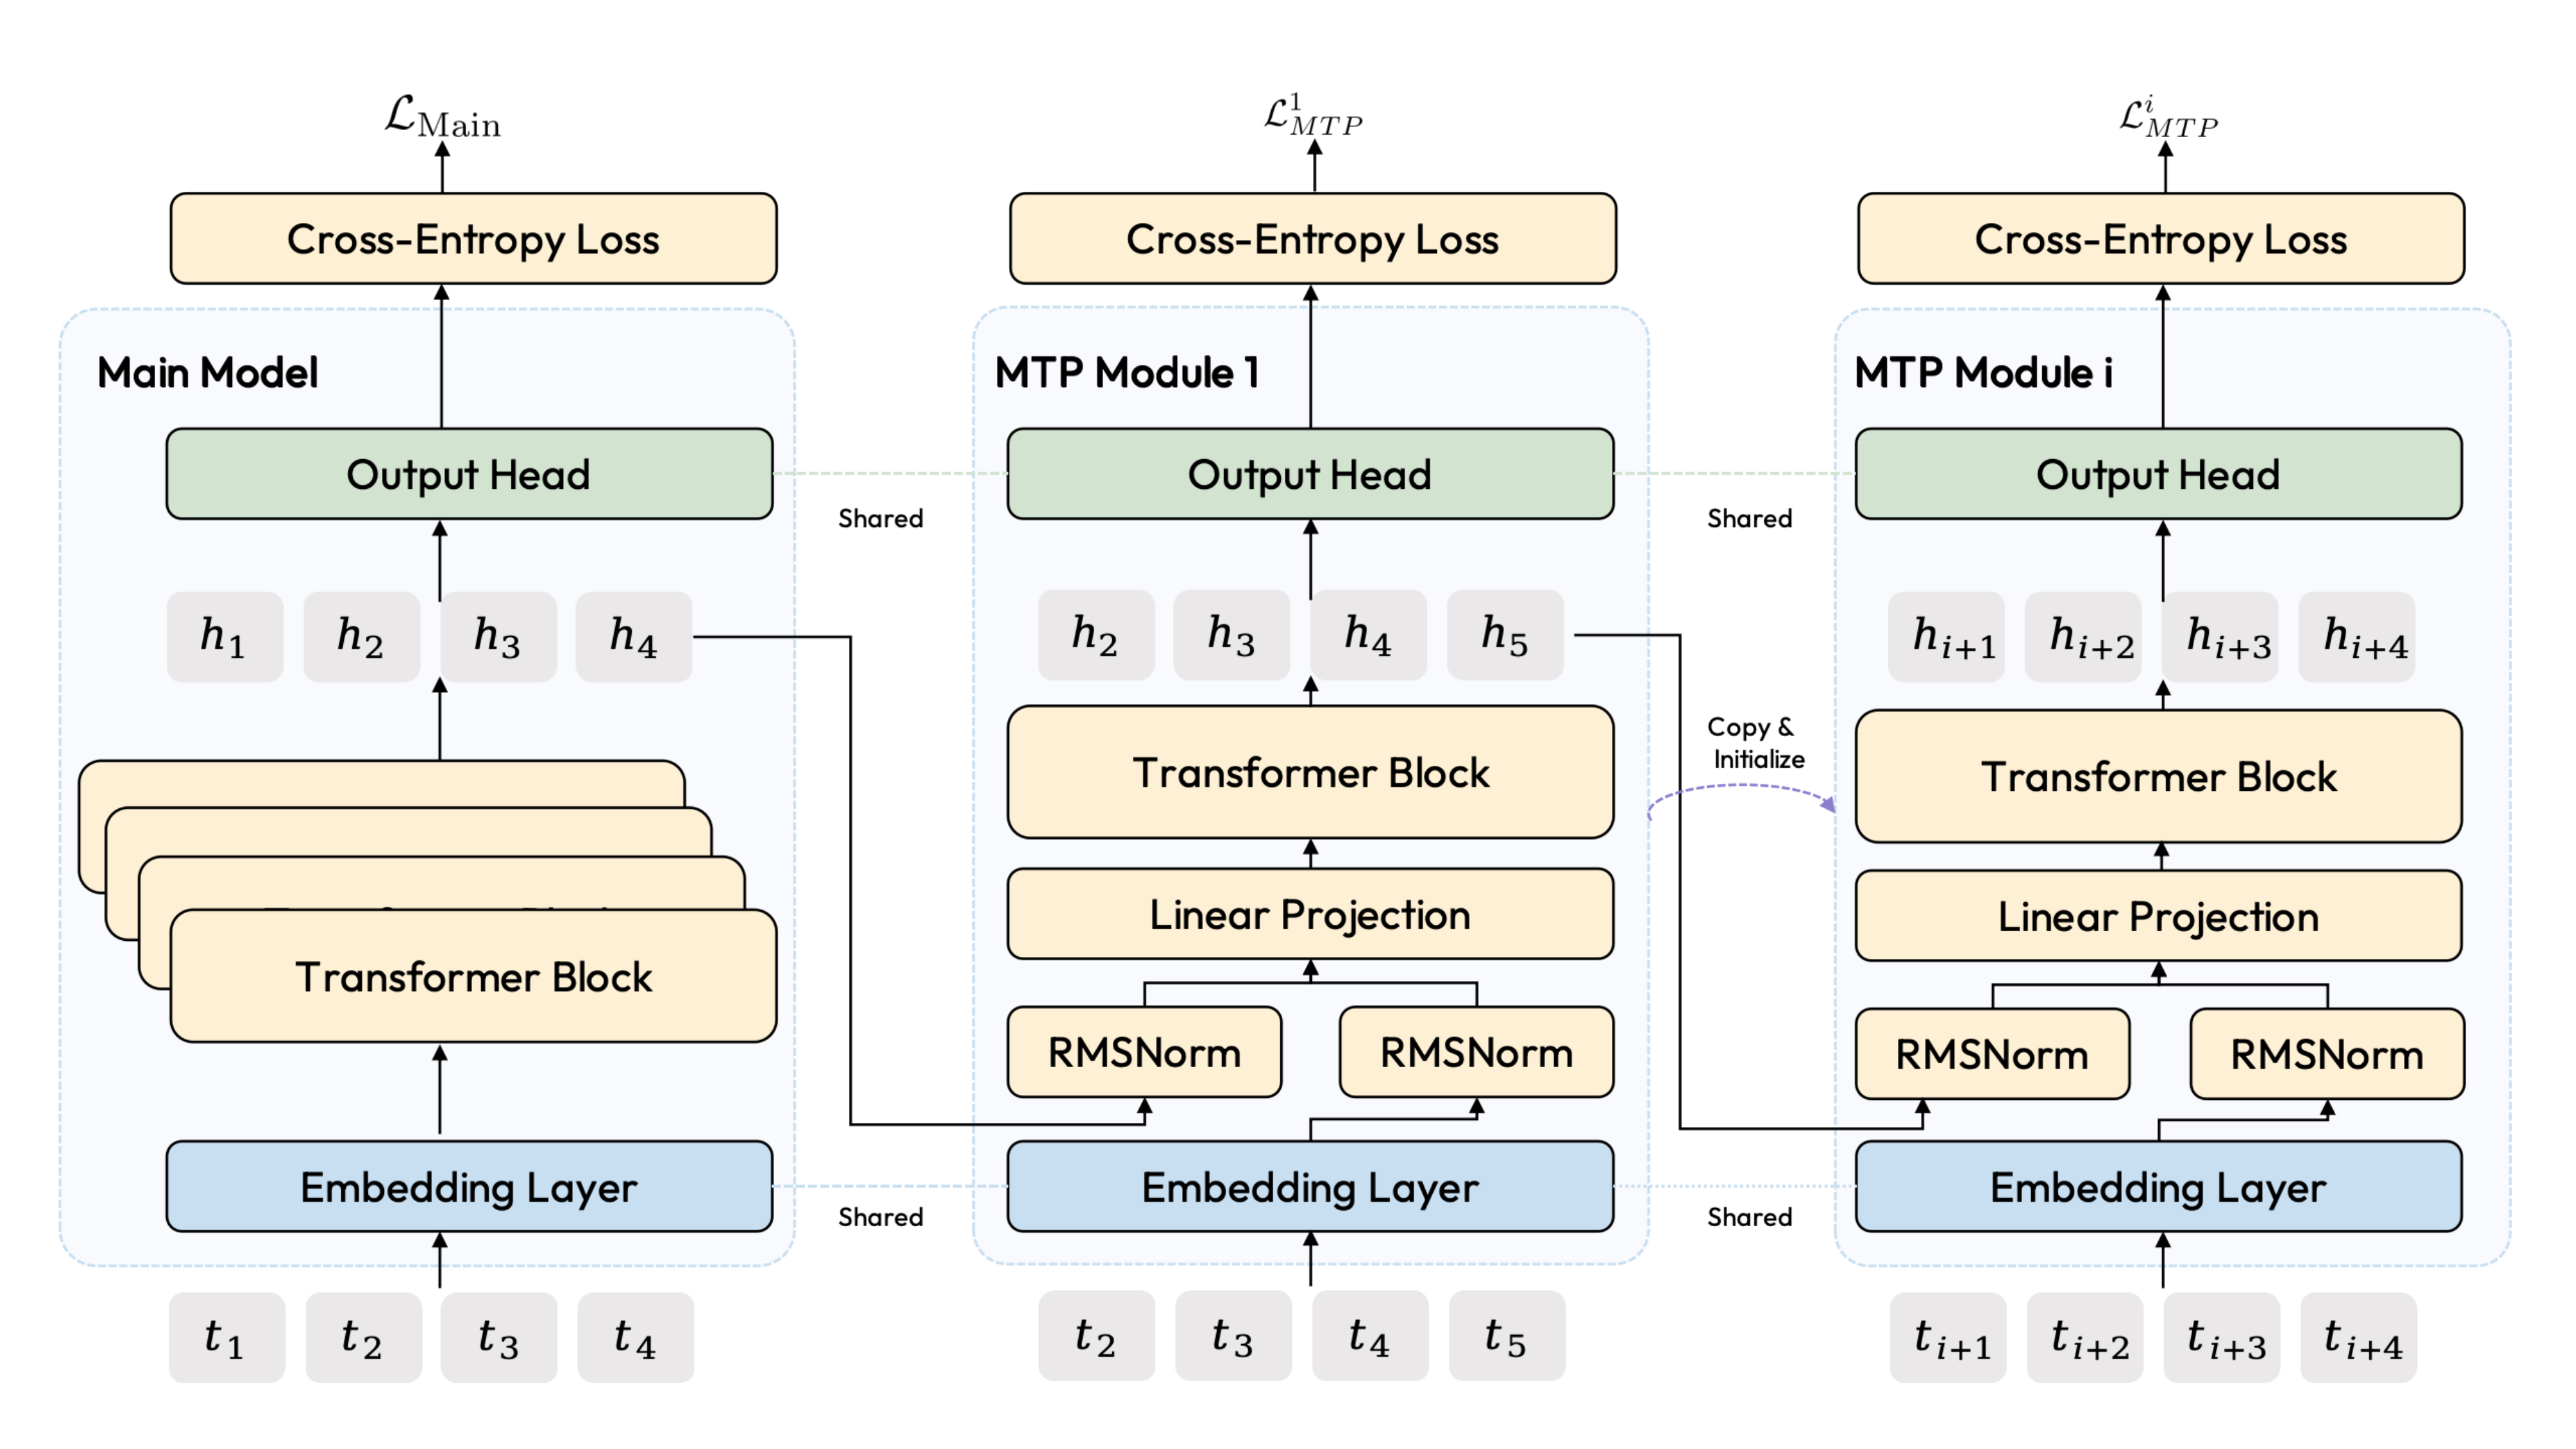
\includegraphics[width=0.85\textwidth]{figures_new/MTP.pdf}
\caption{Multi-Token Prediction (MTP) module architecture used in M2.}
\label{fig:mtp}
\end{figure}

\noindent \textbf{Pre-training Stage.} During pre-training, M2 is trained with a single MTP module ($K=1$) following the design of DeepSeek-V3~\citep{deepseekai2024v3} (Figure~\ref{fig:mtp}), with an initial MTP loss weight of 0.3, which is annealed to 0.1 during the decay phase. As shown in Table~\ref{tab:mtp-ablation}, our ablation indicates that MTP consistently improves model performance across benchmarks, with the largest gains on reasoning-heavy tasks.

\noindent \textbf{Expansion via Weight Copying.} To support multi-step speculative decoding, we expand from one to three MTP modules ($K=3$) during the decay phase of continued pre-training. Rather than random initialization, we copy weights from the main model to initialize the MTP modules. This strategy is critical for two reasons: (1) copy-initialized modules converge significantly faster than randomly initialized ones, which otherwise start with high loss and temporarily degrade the main model; (2) it minimizes disruption to the main model representations during the transition. After expansion, we first freeze the main model and train only the MTP modules for a short period until their loss stabilizes, then switch to joint training of all modules. We also explored keeping the main model frozen throughout, but found that the MTP modules converged to a worse final quality under this MTP-only schedule than under joint training.

\noindent \textbf{Inference.} At inference time, the three MTP modules generate draft tokens that are verified by the main model in a single forward pass, providing throughput improvement while maintaining identical output quality to standard autoregressive decoding.
